% === Cours de Java

\subsection{Organiser le code}

\imgfullw{../img/fruitetlegumes.jpg}
	{
		\begin{flushright}
		\vspace{1cm}
		\LARGE\bf\color{white}
		Rangement
		\vspace{-1cm}
	\end{flushright}
	}
	{https://www.flickr.com/photos/wien/418840561}

\begin{frame}{Le groupement en package}
	Toutes les classes de l'\emph{API} Java sont regroup�es logiquement \dots 
	en \emph{package}
	\bigskip
\begin{center}
  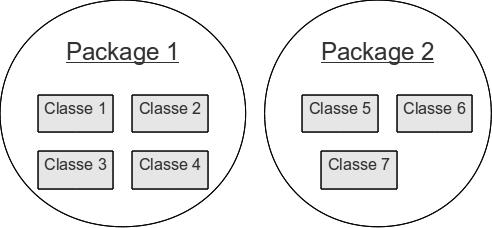
\includegraphics[scale=.6]{../img/package}
\end{center}
\end{frame}

\begin{frame}{La notion de package}
Un \emph{package} donne un nom complet � une classe
\begin{itemize}
    \item {\java|mon.paquet.MaClasse|},
    \item {\java|be.heb.esi.java1.MaClasse|}, 
    \item {\java|java.util.Scanner|},
	\item {\java|org.apache.struts2.components.Anchor|}
  \end{itemize} 
\end{frame}

\begin{frame}[fragile]{Utilisation}
Pour utiliser une classe 
\begin{itemize}
\item mettre le nom \emph{qualifi�} (complet)
\begin{Java}
  java.util.Calendar now = java.util.Calendar.getInstance();
\end{Java}
\item ou utiliser \java{import} qui cr�e un raccourci
\begin{Java}[basicstyle=\scriptsize]
  import java.util.Calendar;
  public Test {
  ...
    Calendar now = Calendar.getInstance();
  ...
  }
\end{Java}
\end{itemize}
\textbf{Cas particulier} Le package \java|java.lang| est import� implicitement
\end{frame}

\begin{frame}{Utilisation}
Comment savoir comment utiliser les classes et m�thodes ? 
\bigskip
\begin{flushright}
	En lisant la \emph{javadoc}
\end{flushright}
\end{frame}

\imgfullh{../img/api}{}
{(http://download.oracle.com/javase/7/docs/api/)}

\begin{frame}{Utilisation}
On peut y lire le nom du package 
\begin{center}
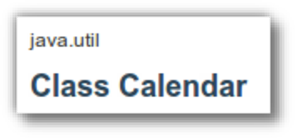
\includegraphics[scale=.6]{../img/api-package}
\end{center}
et la description de la m�thode
\begin{center}
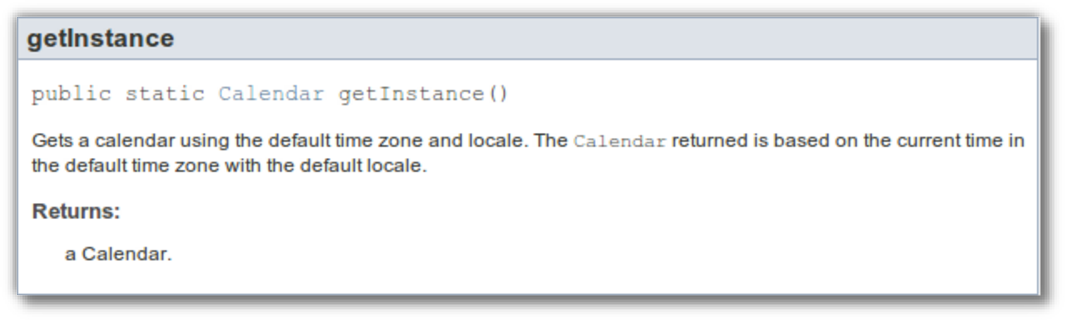
\includegraphics[scale=.6]{../img/api-methode}
\\{\small \textit{On verra comment produire une \emph{javadoc} similaire pour son code}}
\end{center}
\end{frame}

\full[bluepigment]{
	\begin{center}
		\Large\bf\color{azuremist}
		Comment cr�er mes propres \textit{packages} ?
	\end{center}
}

\begin{frame}[fragile]{Cr�er ses packages}
	Commande: \java|package <nom du paquet>|
	\bigskip
\begin{Java}
package be.heb.esi.java1;
public class Test { 
  // Nom complet : be.heb.esi.java1.Test
}
\end{Java}
\end{frame}

\begin{frame}[fragile]{Cr�er ses packages}
Qu'est-ce qui va changer en pratique ?
\begin{itemize}
\item La compilation ne change pas : 
 \begin{Java}
 javac NomClasse.java
 \end{Java}
\item L'ex�cution change : 
 \begin{Java}
 java nom.paquet.NomClasse
 \end{Java}
\end{itemize}
\bigskip
Cela a une incidence sur l'endroit o� placer le \emph{bytecode}
\end{frame}

\imgfullh{../img/api}
{	
	\color{bluepigment}\Large\bf
	\colorbox{aliceblue}{%
		\parbox{.95\linewidth}{%
		\centering Connaitre l'API,\\ c'est gagner du temps ! }
	}
}
{(http://download.oracle.com/javase/7/docs/api/)}


